\documentclass[11pt]{article}
\usepackage{fullpage}
\usepackage{setspace}
\usepackage{amsmath}
\usepackage{fancyvrb}
\usepackage{enumerate}
\usepackage{pgfplots}
\usepackage{graphicx}
\usepackage{float}
\usepackage{multirow}

\begin{document}
\noindent\large{Math 5365}\\
\large{Data Mining 1}\\
\large{Homework 3}\\
\large{Mary Barker}
\newline

\begin{enumerate}
\item The \verb|kyphosis| data set in R contains information about 
children who have had corrective spinal surgery.

The data is stored for 81 subjects, with 4 columns for each. The 
columns are Kyphosis which takes values `absent' or `present', 
Age (in months), Number, which gives the number of vertebrae involved 
and Start, which is the topmost vertebra number operated on. 

\item the tree for predicting Kyphosis based upon the other variables 
in the data set is shown below. 
\begin{center}
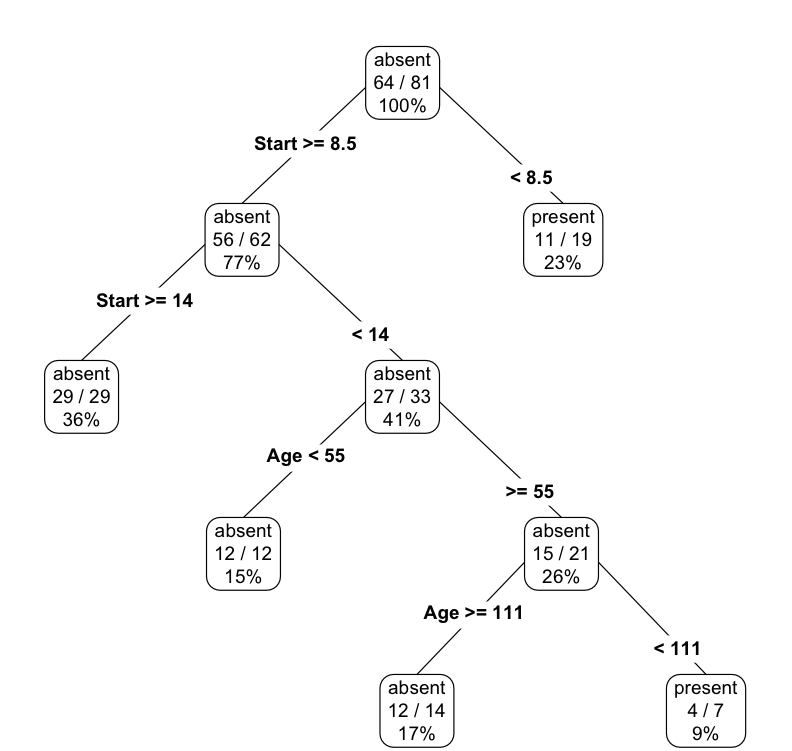
\includegraphics[scale=0.35]{nicetree}
\end{center}

The confusion matrix is shown below.

\begin{center}
\begin{tabular}{  c   c | c | c |}
\cline{3-4}
& & \multicolumn{2}{ c|}{predicted kyphosis}\\
\cline{3-4}
& & absent & present\\
\cline{1-4}
\multicolumn{1}{|c|}{
\multirow{2}{*}{Kyphosis}} & 
\multicolumn{1}{ |c| }{absent} & 53 & 11 \\ \cline{2-4}
\multicolumn{1}{ |c  }{} &
\multicolumn{1}{ |c| }{present} & 2 & 15 \\ \cline{1-4}
\end{tabular}
\end{center}

The accuracy is the sum of the diagonal entries of the decision matrix (in 
other words, the number of accurate predicted results) divided by the total 
number. For this case, 
accuracy = 0.8395062

The error is 
error = 1 - accuracy = 0.1604938

\item According to the tree, the most important variables for predicting 
kyphosis are Start, which is the vertebra being operated on and the 
Age of the patient. 
These two variables partition the data most effectively. 

\begin{center}
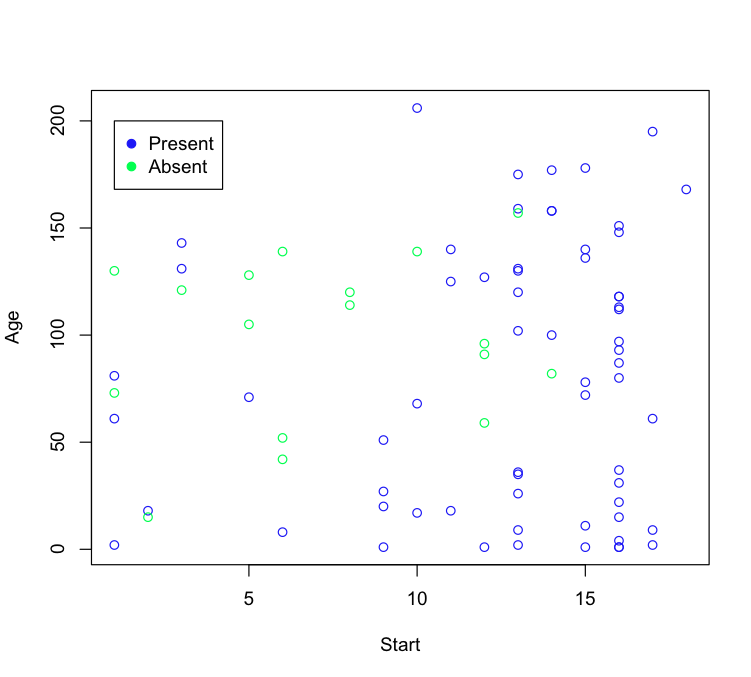
\includegraphics[scale=0.35]{scatterplot}
\end{center}

\item For the simple tree case using the ctree command, the tree was 
generated as shown. 

\begin{center}
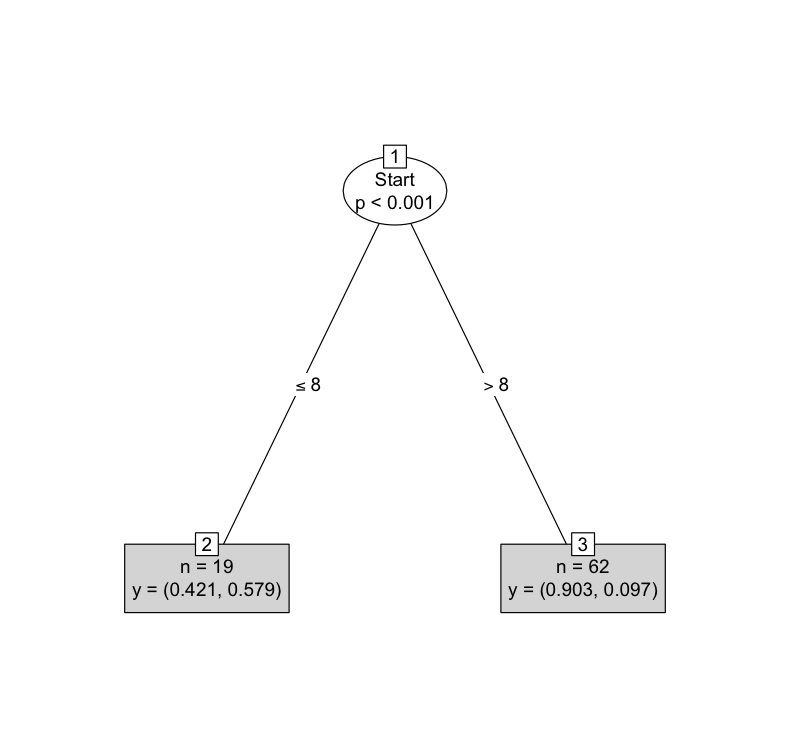
\includegraphics[scale=0.35]{simpletree}
\end{center}

The confusion matrix for this case is 

\begin{center}
\begin{tabular}{  c   c | c | c |}
\cline{3-4}
& & \multicolumn{2}{ c|}{predicted kyphosis}\\
\cline{3-4}
& & absent & present\\
\cline{1-4}
\multicolumn{1}{|c|}{
\multirow{2}{*}{Kyphosis}} & 
\multicolumn{1}{ |c| }{absent} & 56 & 8 \\ \cline{2-4}
\multicolumn{1}{ |c  }{} &
\multicolumn{1}{ |c| }{present} & 6 & 11 \\ \cline{1-4}
\end{tabular}
\end{center}
The accuracy and error for this confusion matrix are:  
accuracy = 0.8271605
, and 
error = 1 - accuracy = 0.1728395

%5
\item 
The main difference between the two trees is in the number and 
distribution in the end nodes. The simple tree has fewer terminal 
nodes, which gives a simpler categorization. In addition, the distribution 
in the right node is close to pure (roughly 90\% ). However, the 
distribution in the left node is very impure, closer to $50\%$. This is 
where the more complex tree is better. Therefore the answer to which is 
the better tree is problem dependent. The simple tree is best for 
quick categorization for when Start > 8, and the other tree for more 
detailed examination of the data. 

The confusion matrices demonstrate a similar breakdown of effectiveness. 
Using the information to calculate error and accuracy shows that the 
rpart tree shows a slightly higher accuracy. However, the difference in 
accuracy is so small as to be negligible. 

%6
\item 
The overall entropy of the system is 0.7412467. 

The rpart tree had a weighted entropy of 
0.4177394.

The ctree had a weighted entropy of 
0.5819756.

%7
\item There is no great difference between the two trees. 
The maximum petal length for setosa flowers was recorded in 
the table as 1.9, and the minimum length petal for veriscolor 
was recorded as 3.0.

Therefore the initial split requirement for the tree on page 28 
(which is length $\le$ 2.4) splits all of the setosa flowers into one branch. 
The $p$ values in that branch show that neither virginica nor versicolor 
flowers are included in that branch, but are completely in the other. 
This is exactly the same condition in its effect upon the distribution as 
the condition on page 38 for length $\le 1.9$, since all setosa petals are 
less than or equal to 1.9, and all other flower types have petals greater than 2.4.

The code used to calculate the minimum and maximum lengths of the respective flower 
types is shown below.

\begin{Verbatim}[numbers=left]
sindex=(iris$Species == "setosa")
largest_length = max(Petal.Length[sindex])
largest_length

vindex=(iris$Species == "versicolor")
shortest_length = min(Petal.Length[vindex])
shortest_length
\end{Verbatim}

\end{enumerate}

The code for the kyphosis related questions is shown below. 

\begin{Verbatim}[numbers=left]
# Data Mining hw 3

# problem 1
##kyphosis {rpart}
#it is a data frame with 81 rows, 4 columns representing data on children 
#who have had corrective spinal surgery.
#
#columns are as follows:
#+ Kyphosis
#+ + + A factor with levels 'absent' 'present' indicating if a kyphosis was 
#+ + + present after the operation
#
#
#+ Age
#+ + + in months
#
#+ Number 
#+ + + the number of vertebrae involved
#
#+ Start
#+ + + The number of the first (topmost) vertebra operated on.
#
library(rpart)
library(rpart.plot)
library(party)
library(treemap)
attach(kyphosis)

# problem number 2
#a)
ktree=rpart(Kyphosis~Age+Number+Start,data=kyphosis)
plot(ktree,main="Kyphosis~Age+Number+Start")
prp(ktree,type=2,extra=104)
#b)
predkyphos = predict(ktree,newdata=kyphosis,type="class")
confusionmatrix=table(Kyphosis,predkyphos)
#c)
accuracy = sum(diag(confusionmatrix))/sum(confusionmatrix)
error = 1 - accuracy

# problem number 4
#a)
ktree2=ctree(Kyphosis~.,data=kyphosis)
plot(ktree2,type='simple')
#b)
predkyphos2 = predict(ktree2,newdata=kyphosis)
confusionmatrix=table(Kyphosis,predkyphos2)
#c)
accuracy = sum(diag(confusionmatrix))/sum(confusionmatrix)
error = 1 - accuracy
\end{Verbatim}
\end{document}
